\maketitle
\tableofcontents
\newpage

\section{Первое задание}

\paragraph{Текст задания} ~\\
(а)Представить слагаемые и результат в виде нормализованного числа с плавающей точкой двойной точ-ности: $(-1)^{s}(2^{e-1023})(1.f)$, где $1.f$ записанов двоичном виде.(б) Если результат неточный (не умещается целиком в мантиссе), то указать относительную погрешность ошибки. Исходные данные в десятичной системе счисления.

 \[ -1593.5859375 \cdot 2^{128} + 1619.09765625 \cdot 2^{141}\]

\paragraph{Решение} ~\\
Для начала разберемся с первым числом $-1593.5859375 \cdot 2^{128}$:
\begin{align*}
 %первое выражение
  -1593.5859375_{10}& = 11000111001.1001011_{2} = 1.10001110011001011_{2} \cdot 2^{10} \\[1mm]
%второе выражение
  -1593.5859375_{10} \cdot 2^{128}& = (-1)^{1}(2^{1161-1023}) \cdot 1.10001110011001011
\end{align*}
$s = 1$, $e = 1023+128+10 = 1161$, $f = 1000111001100101\underbrace{0\ldots0_{\text{35 нулей}}}$\\[1em]
Теперь нормализуем $1619.09765625 \cdot 2^{141}$:
\begin{align*}
%первое выражение
  1619.09765625_{10}& = 11001010011.00011001_{2} = 1.100101001100011001_{2} \cdot 2^{10} \\[1mm]
%второе выражение
  1619.09765625 \cdot 2^{141}& = (-1)^{0}(2^{1174-1023})(1.100101001100011001)
\end{align*}
$s = 0$, $e = 1023 + 141 + 10 = 1174$, $f = 100101001100011001\underbrace{0\ldots0_{\text{34 нуля}}}$\\[1em]

\begin{multline*}
  11001010011.00011001 \cdot 2^{141}  - 11000111001.10001011 \cdot 2^{128} = \\[3mm]
  = 2^{141} (11001010011.00011001 - 11000111001.1001011 \cdot 2^{-13}) = \\[3mm]
  = 2^{141} (11001010011.00011001 - 0,\underbrace{0\ldots0_{\text{12 нулей}}}\underbrace{110001110010001011_{\text{18 битов}}}) = \\[3mm]
  = 2^{141} (\underbrace{11001010011.00011001_{\text{19 битов}}}\underbrace{\empty_{\text{5 битов}}}\underbrace{\empty_{\text{18 битов}}})
\end{multline*}
Получается 42 бита $\Rightarrow$ число полностью поместится, а значит никакой погрешности нет.

\section{Второе задание}

\paragraph{Текст задания} ~\\
Написать последовательность инструкций Matlab, формирующих указанную матрицу. Около каждой инструкции указать промежуточный результат в виде матрицы. Разрешается использовать матричные функции(eye, repmat, flipud и др.). Использовать циклы нельзя.\\[1em]
Входные данные: Целое $n \geq 20$\\[1em]
Надо получить:
\[
  \begin{pmatrix}
    0 & 1 & 0 & 2 & 0 & 3 & 0 & \cdots & n \\
    0 & 1 & 0 & 2 & 0 & 3 & 0 & \cdots & n \\
    \vdots & \vdots & \vdots & \vdots & \vdots & \vdots & \vdots & \ddots & \vdots \\
    0 & 1 & 0 & 2 & 0 & 3 & 0 & \cdots & n \\
    0 & 1 & 0 & 2 & 0 & 3 & 0 & \cdots & n
  \end{pmatrix}
  \} \text{2n строк}
\]

\paragraph{Решение} ~\\
\begin{lstlisting}
  n = input();
  A \[= [1 : 0.5 : n]
  \end{lstlisting}
\[A = 1.00, 1.50, 2.00, 2.50, 3.00, 3.50, 4.00, \ldots, n\]

\begin{lstlisting}
  A = fix(A)
\end{lstlisting}
\[A = 1, 1, 2, 2, 3, 3, 4, 4, 5, 5, \ldots, n\]

\begin{lstlisting}
  A = [0, A]
\end{lstlisting}
\[A = 0, 1, 1, 2, 2, \ldots, n\]

\begin{lstlisting}
  A = repmat(A, 2*n, 1);
\end{lstlisting}
\[
  A =
  \begin{pmatrix}
    0 & 1 & 1 & 2 & 2 & 3 & 3 & \cdots n \\
    0 & 1 & 1 & 2 & 2 & 3 & 3 & \cdots n \\
    \vdots & \vdots & \vdots & \vdots & \vdots & \vdots & \vdots & \ddots & \vdots \\
    0 & 1 & 1 & 2 & 2 & 3 & 3 & \cdots n
  \end{pmatrix}
  \} \text{2n строк}
\]

\begin{lstlisting}
  X = [0, 1]
  X = repmat(X, 2*n, 1)
\end{lstlisting}
\[
  X =
  \begin{pmatrix}
    0 & 1 \\
    \vdots & \vdots \\
    0 & 1
  \end {pmatrix}
  \} 2n
\]

\begin{lstlisting}
  X = repmat(X, 1, n)
\end{lstlisting}
\[
  X =\underbrace{
  \begin{pmatrix}
    0 & 1 & 0 & 1 & \cdots & 1 \\
    0 & 1 & 0 & 1 & \cdots & 1 \\
    \vdots & \vdots & \vdots & \vdots & \ddots & \vdots \\
    0 & 1 & 0 & 1 & \cdots & 1
  \end{pmatrix}
}_{\text{n столбцов}} \}\text{2n строк}
\]

\begin{lstlisting}
  A = A.*X
\end{lstlisting}
\[
  A =
  \begin{pmatrix}
    0 & 1 & 0 & 2 & 0 & 3 & 0 & \cdots & n \\
    0 & 1 & 0 & 2 & 0 & 3 & 0 & \cdots & n \\
    \vdots & \vdots & \vdots & \vdots & \vdots & \vdots & \vdots & \ddots & \vdots \\
    0 & 1 & 0 & 2 & 0 & 3 & 0 & \cdots & n \\
    0 & 1 & 0 & 2 & 0 & 3 & 0 & \cdots & n
  \end{pmatrix}
\]

% ------------------------------------------------------------------------------------------------
% Третье задание
% ------------------------------------------------------------------------------------------------
\section{Третье задание}

\paragraph{Текст задания} ~\\
(а) Локализовать корни уравнения (для каждого корня $z_{i}$ указать отрезок $[a_{i}, b_{i}]$, содержащий только один этот корень$z_{i}$). Для \textit{\textsl{каждого}} корня (б) построить итерационный процесс $x_{n+1} = \varphi(x_{n})$, сходящийся к корню и (в) указать начальное значение $x_{0}$. Указание: локализацию проводить перебором интервалов $[a_{i}, b_{i}]$ или средствами математического анализа.\\[2mm]
\[4x^{3} - 6x + 1 = 0\]

\paragraph{Решение} ~\\[3mm]
\begin{tabular}{| c | c | c | c | c | c | c | c |}
  \hline
  $x$ & -3 & -2 & -1 & 0 & 1 & 2 & 3 \\
  \hline
  $f(x)$ & -89 & -19 & 3 & 1 & -1 & 21 & 91 \\
  \hline
  $sign(f(x))$ & - & - & + & + & - & + & + \\
  \hline
\end{tabular}\\[2mm]
Можно увидеть как $f(x)$ меняет знак при $x = -2 \rightarrow -1$ и при $x = 0 \rightarrow 1$ и $x = 1 \rightarrow 2$, то есть: $a_{1} = -2, b_{1} = -1; a_{2} = 0, b_{2} = 1; a_{3} = 1, b_{3} = 2$.\\[3mm]
Найдем итерационный процесс для отрезка $\left[-2, -1\right]$:\\
Воспользуемся методом Ньютона:\\
Для этого найдем производную: $f^{'}(x) = 12x^{2}-6$
\[
  x_{n+1} = x_{n} - \frac{f(x)}{f^{'}(x)} = x_{n} - \frac{4x_{n}^{3}-6x_{n}+1}{12x_{n}-6} = \frac{-4x_{n}^{3}+12x_{n}^{2}-1}{12x_{n}-6}
\]
Так как $f^{'} < 0$ и $f^{''} < 0$ на промежутке $\left[-2, 1\right]$, то $x_{0} = -1$.\\[3mm]
Найдем итерационный процесс для отрезка $\left[ 0, 1\right]$:\\
% TODO: написать итерационный процесс для этого промежутка
По методу Ньютона $x_{0}$ для этого отрезка $x_{0} = 1$

Найдем итерационный процесс для отрезка $\left[1, 2 \right]$:\\
\begin{gather*}
  4x^{3}-6x+1 = 0 \\
  x^{3} = \frac{6x-1}{4} \\
  \varphi(x) = x = \left(\frac{6x-1}{4}\right)^{\frac{1}{3}} \\
  \varphi^{'}(x) = \frac{\sqrt[3]{2}}{(6x-1)^{\frac{2}{3}}} \\
  |\varphi^{'}(x)| < 1 \\
  |\frac{3\sqrt{2}}{(6x-1)^{\frac{2}{3}}}| < 1 \\
\end{gather*}
Решение этого неревенства: $\left(0.4, \infty \right) (\supseteq \left[1, 2\right])$
\begin{gather*}
  x_{n+1} = \frac{3\sqrt{2}}{(6x-1)^{\frac{2}{3}}} \\
  x_{0} \in \left[1, 2 \right] \\
  x_{0} = 2
\end{gather*}


% ------------------------------------------------------------------------------------------------
% Четвертое задание
% ------------------------------------------------------------------------------------------------
\section{Четвертое задание}

\paragraph{Текст задания} ~\\
Известно, что интервалу $\left[a, b\right]$ принадлежит \textit{\textsl{только}} корень $x_{*}$ уравнения (другие корни интервалу не принадлежат). (а) Построить итерационный процесс Ньютона $x_{n+1} = x_{n} -f(x_{n})/f^{'}(x_{n})$ и (б) обосновать какую из границ интервала $\left[a, b\right]$ можно принять за $x_{0}$. Указание: в пункте (б) выяснить знаки производных $f^{'}(x)$ и $f^{''}(x)$ и использовать соотвествующую теорему.\\[3mm]
\[
  x - \frac{e^{x}}{x} + \frac{3}{2} = 0, x_{*} \in \left[1, 3; 1, 4\right]
\]

\paragraph{Решение} ~\\
\[
  f^{'}(x) = \frac{x^{2}-xe^{x}+e^{x}}{x^{2}}
\]\\[1mm]
Итерационный процесс Ньютона:
\[
  x_{n+1} = x_{n} - \frac{f(x_{n})}{f^{'}(x_{n})} = \frac{(2x+2e^{x}+3x)x}{2(x^{2}-xe^{x}+e^{x})}
\]
Теорема справедлива если на всем отрезке $\left[a, b\right]$ выполняются:\\
(1) $f^{'} > 0, f^{''} > 0, x_{0} = b$\\
(2) $f^{'} < 0, f^{''} < 0, x_{0} = a$\\
(3) $f^{'} < 0, f^{''} < 0, x_{0} = b$\\
(4) $f^{'} > 0, f^{''} < 0, x_{0} = a$\\
\begin{gather*}
  f^{'}(x) = \frac{x^{2}-xe^{x}+e^{x}}{x^{2}} \\
  f^{''}(x) = -\frac{e^{x}(x^{2}-2x+2)}{x^{3}}
\end{gather*}
$f^{'}(x)$ --- положительна, а $ f^{''}(x)$ --- отрицательна на всем отрезке $\left[a, b\right]$ $\Rightarrow$ теорема применима
\begin{gather*}
  f^{'}(1.3) > 0 \\
  f^{''}(1.3) < 0 \Rightarrow x_{0} = 1.3
\end{gather*}

% ------------------------------------------------------------------------------------------------
% Пятое задание
% ------------------------------------------------------------------------------------------------
\section{Пятое задание}

\paragraph{Текст задания} ~\\
(а) Построить интерполяционный многочлен Лагранжа для функции $f(x)$ по узлам $x_{i}$. (б) Оценить сверху погрешность $|R_{n}(x)|$ приближения функции многочленом.\\[2mm]
\[
  \ln(x) - \sqrt{x}, x_{0} = 3, x_{1} = 4, x_{2} = 5
\]

\paragraph{Решение} ~\\

\begin{tabular}{|c | c | c | c|}
  \hline
  $x$ & 3 & 4 & 5 \\
  \hline
  $f(x)$ & 0.46 & 0.48 & 0.47 \\
  \hline
\end{tabular}

Найдем многочлен Лагранжа, для:
\begin{multline*}
  L(x) = y_{0} \frac{(x - x_{1})(x - x_{2})}{(x_{0} - x_{1})(x_{0} - x_{2})} + y_{1} \frac{(x - x_{0})(x - x_{2})}{(x_{1} - x_{0})(x_{1} - x_{2})} + y_{2} \frac{(x - x_{0})(x - x_{1})(x - x_{2})}{(x_{2} - x_{0})(x_{2} - x_{1})} = \\[3mm]
  = 0.46 \frac{(x - 4)(x - 5)}{-1 \cdot (-2)} + 0.48 \frac{(x - 3)(x-5)}{1 \cdot (-1)} + 0.47 \frac{(x - 3)(x-4)}{2} = \\[3mm]
  = 0.2325(x^{2}-9x+20) - 0.484(x^{2}-8x+15) + 0.236(x^{2}-7x+12) = \\[3mm]
  = -0.0155x^{2} + 0.1275x + 0.222
\end{multline*}\\[2mm]
Окончальтельно получаем, что наш интерполяционный многочлен равен $L(x) = -0.0155x^{2} + 0.1275x + 0.222$. Проверим это с помощью матлаба, на рисунке~\ref{fig:plot_5}
\lstinputlisting{code/task_5.m}
\begin{figure}
  \caption{Красный график это наша функция, а черный - полином Лагранжа.}
  \label{fig:plot_5}
  \centering
  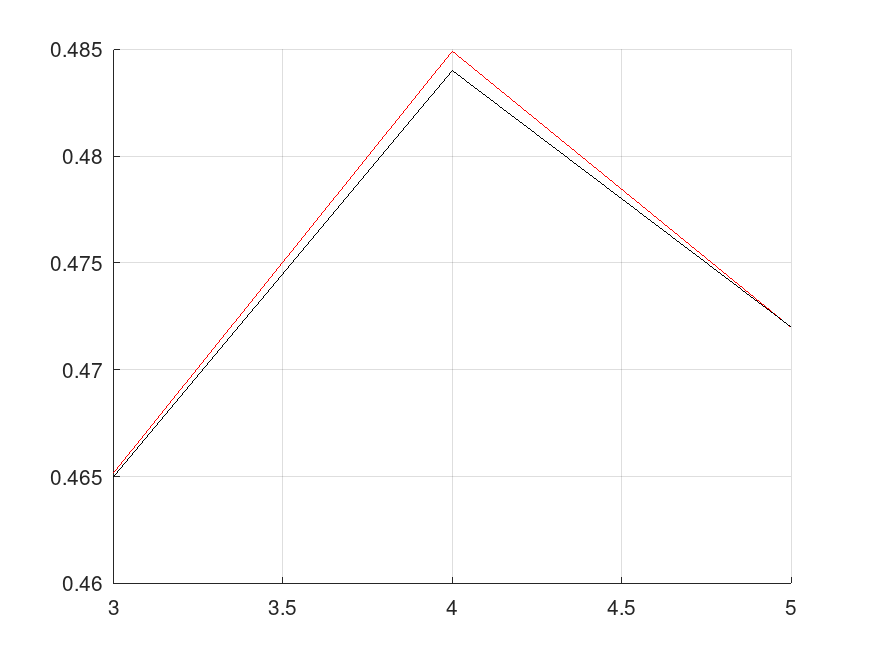
\includegraphics[width=0.8\textwidth]{images/task_5.png}
\end{figure}

Теперь найдем погрешность $|R_{2}(x)|$:\\[2mm]
\begin{align*}
  |R_{2}(x)| &= \frac{f^{(3)}(x)}{3!}(x-x_{0})(x-x_{1})(x-x_{2}) \\[1mm]
  |R_{2}(x)| & \leq \frac{M_{3}}{3!}(x-x_{0})(x-x_{1})(x-x_{2}) \\[1mm]
  M_{3} &= \max_{\left[a, b\right]}|f^{(3)}(x)| \\[1mm]
  f^{(3)}(x) & = \frac{2}{x^{3}} - \frac{3}{8x^{5/2}}
\end{align*}
Максимум $f^{(3)}(x)$ на отрезке $[3, 5]$, достигается в точке $3$.
\begin{gather*}
  f^{(3)}(x) = 0.05 \\[1mm]
  |R_{2}(x)| \leq \frac{0.05}{6}(x-3)(x-4)(x-5) \leq \frac{1}{120}x^{3} - \frac{1}{10}x^{2} + \frac{47}{120}x - \frac{1}{2}
\end{gather*}

% ------------------------------------------------------------------------------------------------
% Шестое задание
% ------------------------------------------------------------------------------------------------
\section{Шестое задание}

\paragraph{Текст задания} ~\\
Заданную функцию будут интерполировать на отрезке $\left[a, b\right]$ по чебышёвским узлам с заданной точностью $|R_{n}(x) < \epsilon|$. Требуется (а) определить требуемое для заданной точности $\epsilon$ количество узлов (т.е. степень интерполяционного многочлена плюс 1) и (б) вычислить значения всех узлов и отметить их на действительной оси $Ox$ (если узлов окажется много, ограничиться вычислением значений наименьших 10 узлов).\\[3mm]
\[
  f(x) = x^{2} - \sin\left(\frac{x}{2}\right), \text{на отрезке} \left[\frac{\pi}{4}, \pi\right] \text{с точностью} \epsilon = 10^{-3}
\]

\paragraph{Решение} ~\\
\[
  f^{'''}(x) = \frac{1}{8}\cos(\frac{x}{2})
\]
Сначала найдем кол-во узлов для $\epsilon = 10^{-3}$\\[2mm]
Для $n = 2$:
\begin{gather*}
  |R_{2}(x)| \leq \frac{M_{3}}{3!}\cdot\left(\pi - \frac{pi}{4}\right)^{3}\cdot2^{-5}, \text{где} M_{3} = \max_{\left[\pi, \frac{\pi}{4}\right]}|f^{'''}(x)|\\
  M_{3} = \max_{\left[\pi, \frac{\pi}{4}\right]}|f^{'''}(x)| \approx 0.1155 \\
  |R_{2}(x)| = \frac{0.1155}{6} \cdot \left(\frac{3\pi}{4} \right) \approx 7.9 \cdot 10^{-4} = 0.00079 < 0.001 (10^{-3})
\end{gather*}
Степень интерполяции равна двум, значит кол-во узлов равно трем. Теперь требуется вычислить значение узлов и отметить их на действительной оси $Ox$
\[
  x_{k} = \pi \cos\left(\frac{2k-1}{2n}\pi\right)
\]
\begin{lstlisting}
  n = 3;
  k = [1 : n];
  xk = pi * cosd(pi * (2*k-1)/(2*n))
  hold on, grid on
  xlim([xk(1) - 0.01, xk(3) + 0.01])
  line([xk(1) - 0.02, xk(3) + 0.02], [0, 0], 'color', 'k')
  plot(xk, 0, 'r*')
\end{lstlisting}
\begin{lstlisting}[backgroundcolor=\color{cyan}]
  xk =

   3.1413   3.1413   3.1389
\end{lstlisting}
\begin{figure}[h]
  \caption{Чебышевские узлы на оси Ox}
  \label{fig:plot_6}
  \centering
  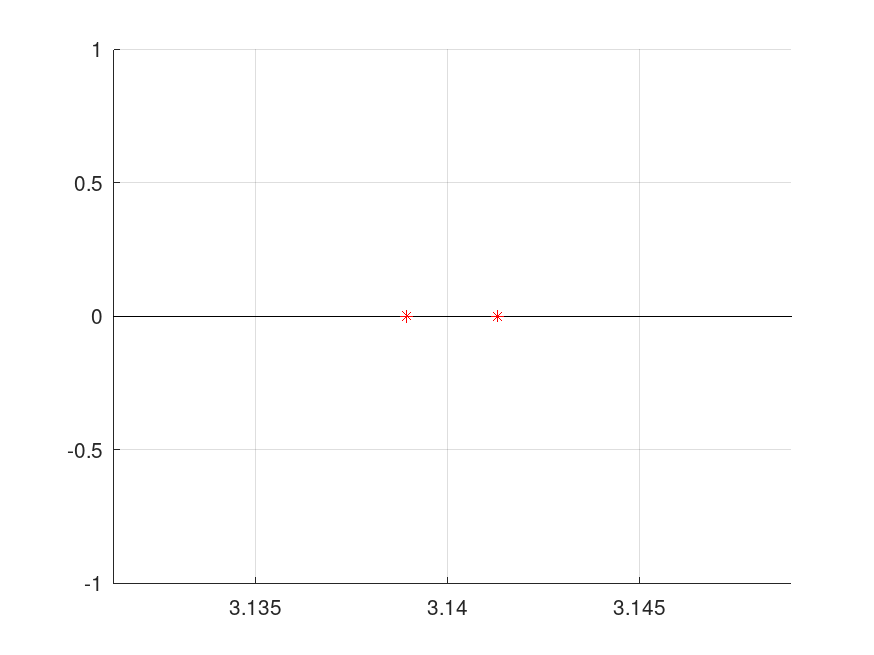
\includegraphics[width=0.8\textwidth]{images/task_6_1.png}
\end{figure}

\section{Седьмое задание}
\paragraph{Текст задания} ~\\
Данные некоторого физического эксперимента представлены в таблице. Характер зависимости $y(x)$ заранее точно неизвестен. Есть предположения, что зависимость может быть линейной, квадратичной или кубической. (а) Методом среднеквадратического приближения построить три типа приближения $y(x)$ (т.е. аппроксимирующие многочлены первой, второй и третьей степеней). (б) Для каждого аппроксимирующего многочлена вычислить среднеквадратическое отклонение $\sqrt{\frac{1}{n+1}\sum_{i=0}^{n}(y(x_{i}) - y_{i})^{2}}$. (в) Выбрать минимальное с.к.о. и указать соответствующий ему тип зависимости (линейная, квадратичная или кубическая), т.е. наиболеевероятный в проведённом эксперименте.

\begin{center}
  \begin{tabular}{ c | c | c | c | c | c }
    $x$ & 2 & 3 & 4 & 5 & 6 \\
    \hline
    $f(x)$ & 17.2 & 45.5 & 96.5 & 175.8 & 288.9
  \end{tabular}
\end{center}

\paragraph{Решение} ~\\
Для апроксемирующего многочлена первой степени воспользуемся такой матрицей:
\[
  \begin{pmatrix}
    n & \sum x_{i}\\
    \sum x_{u} & \sum x_{i}^{2}
  \end{pmatrix}
  \cdot
  \begin{pmatrix}
    a_{1} \\
    a_{2}
  \end{pmatrix}
  =
  \begin{pmatrix}
    \sum y_{i} \\
    \sum x_{i}y_{i}
  \end{pmatrix}
\]

\begin{lstlisting}
  n = 5; %| Кол-во измерений|
  x = [2 : 6];
  y = [17.2, 45.5, 96.5, 175.8, 288.9];

  s(1,1) = n;
  s(2, 1) = sum(x);
  s(1, 2) = s(2, 1);
  s(2, 2) = sum(x.^2)
  b = [sum(y); sum(y*x')]

  a = s\b
  y2 = a(1) + a(2)*x
  hold on; grid on;
  plot(x, y, 'linestyle', 'none', 'marker', 's', 'color', 'r', 'markerfacecolor', 'r');
  plot(x, y2, 'color', 'g');
  legend('|Тест|', '|Апроксимирующая прямая|')
\end{lstlisting}
\begin{lstlisting}[backgroundcolor=\color{cyan}]
  s =

  5   20
  20   90

  b =

  623.90
  3169.30

  a =

  -144.700
  67.370

  y2 =

  -9.9600    57.4100   124.7800   192.1500   259.5200

\end{lstlisting}
\begin{figure}[H]
  \caption{Точки из экспиремента и апроксимирующая прямая (1-ой степени)}
  \label{fig:plot_7_1}
  \centering
  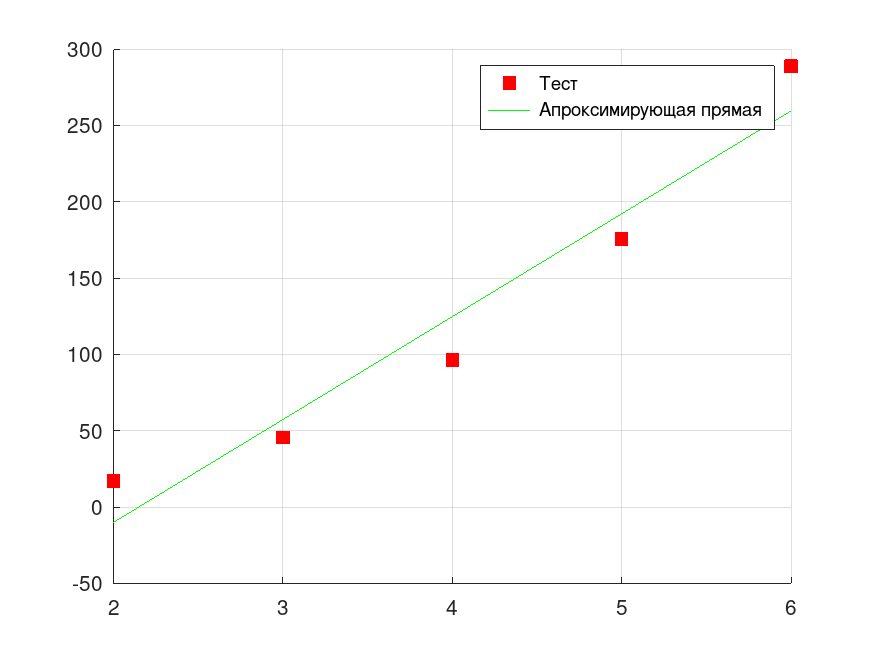
\includegraphics[width=0.8\textwidth]{images/task_7_1.png}
\end{figure}
Среднеквадратичное отклонение:
\[
  \delta = \sqrt{\frac{\sum(y(x)-y_{i})^{2}}{n+1}} \approx 21.64
\]

Для апроксмирующей второй степени:
\[
  \begin{pmatrix}
    n & \sum x_{i} & \sum x_{i}^{2} \\[1em]
    \sum x_{i} & \sum x_{i}^{2} & \sum x_{i}^{3} \\[1em]
    \sum x_{i}^{2} & \sum x_{i}^{3} & \sum x_{i}^{4}
  \end{pmatrix}
  \cdot
  \begin{pmatrix}
    a_{1} \\[1em]
    a_{2} \\[1em]
    a_{3}
  \end{pmatrix}
  =
  \begin{pmatrix}
    \sum y_{i} \\[1em]
    \sum x_{i}y_{i} \\[1em]
    \sum x_{i}^{2}y_{i}
  \end{pmatrix}
\]
\begin{lstlisting}
  n = 5; %| Кол-во измерений|
  x = [2 : 6];
  y = [17.2, 45.5, 96.5, 175.8, 288.9];

  s(1,1) = n;
  s(2, 1) = sum(x);
  s(1, 2) = s(2, 1);
  s(2, 2) = sum(x.^2);

  s(3, 1) = sum(x.^2);
  s(3, 2) = sum(x.^3);
  s(1, 3) = s(3, 1);
  s(2, 3) = s(3, 2);
  s(3, 3) = sum(x.^4)

  b = [sum(y); sum(y*x'); sum(y*x'.^2)]
  a = s\b

  y2 = a(1) + a(2)*x + a(3)*x.^2
  hold on; grid on;
  plot(x, y, 'linestyle', 'none', 'marker', 's', 'color', 'r', 'markerfacecolor', 'r');
  plot(x, y2, 'color', 'g');
  legend('|Тест|', '|Апроксимирующая прямая|')
\end{lstlisting}
\begin{lstlisting}[backgroundcolor=\color{cyan}]
  s =

  5     20     90
  20     90    440
  90    440   2274

  b =

  6.2390e+02
  3.1693e+03
  1.6818e+04

  a =

  53.200
  -45.716
  14.136

  y2 =

  18.311    43.274    96.509   178.014   287.791
\end{lstlisting}
\begin{figure}[H]
  \caption{Точки из экспиремента и апроксимирующая прямая (2-ой степени)}
  \label{fig:plot_7_2}
  \centering
  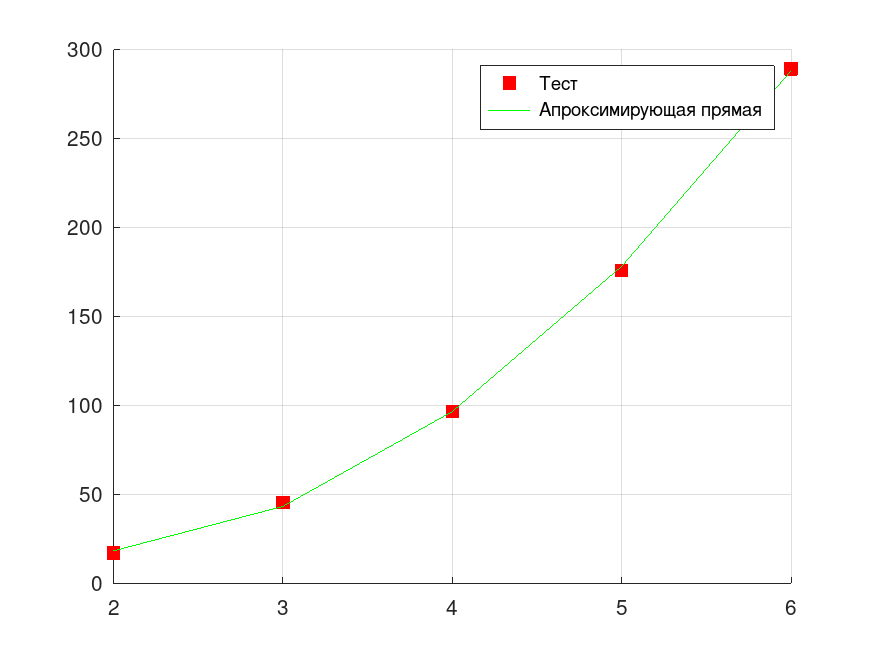
\includegraphics[width=0.8\textwidth]{images/task_7_2.png}
\end{figure}
\[
  \delta \approx 1.4
\]
Для апроксимирующей третей степени:
\[
  \begin{pmatrix}
    n & \sum x_{i} & \sum x_{i}^{2} & \sum x_{i}^{3} \\[1em]
    \sum x_{i} & \sum x_{i}^{2} & \sum x_{i}^{3} & \sum x_{i}^{4} \\[1em]
    \sum x_{i}^{2} & \sum x_{i}^{3} & \sum x_{i}^{4} & \sum x_{i}^{5} \\[1em]
    \sum x_{i}^{3} & \sum x_{i}^{4} & \sum x_{i}^{5} & \sum x_{i}^{6}
  \end{pmatrix}
  \cdot
  \begin{pmatrix}
    a_{1}\\[1em]
    a_{2}\\[1em]
    a_{3}\\[1em]
    a_{4}
  \end{pmatrix}
  =
  \begin{pmatrix}
    \sum y_{i} \\[1em]
    \sum x_{i}y_{i} \\[1em]
    \sum x_{i}^{2}y_{i} \\[1em]
    \sum x_{i}^{3}y_{i}
  \end{pmatrix}
\]
\begin{lstlisting}
  n = 5; %| Кол-во измерений|
  x = [2 : 6];
  y = [17.2, 45.5, 96.5, 175.8, 288.9];

  s(1,1) = n;
  s(2, 1) = sum(x);
  s(1, 2) = s(2, 1);
  s(2, 2) = sum(x.^2);

  s(3, 1) = sum(x.^2);
  s(3, 2) = sum(x.^3);
  s(1, 3) = s(3, 1);
  s(2, 3) = s(3, 2);
  s(3, 3) = sum(x.^4);

  s(4, 1) = sum(x.^3);
  s(1, 4) = s(4, 1);
  s(4, 2) = sum(x.^4);
  s(2, 4) = s(4, 2);
  s(4, 3) = sum(x.^5);
  s(3, 4) = s(4, 3);
  s(4, 4) = sum(x.^6)

  b = [sum(y); sum(y*x'); sum(y*x'.^2); sum(y*x'.^3)]
  a = s\b

  y2 = a(1) + a(2)*x + a(3)*x.^2 + a(4)*x.^3
  hold on; grid on;
  plot(x, y, 'linestyle', 'none', 'marker', 's', 'color', 'r', 'markerfacecolor', 'r');
  plot(x, y2, 'color', 'g');
  legend('|Тест|', '|Апроксимирующая прямая|')
\end{lstlisting}
\begin{lstlisting}[backgroundcolor=\color{cyan}]
  s =

  5      20      90     440
  20      90     440    2274
  90     440    2274   12200
  440    2274   12200   67170

  b =

  6.2390e+02
  3.1693e+03
  1.6818e+04
  9.1920e+04

  a =

  6.5800
  -4.4607
  3.0357
  0.9250

  y2 =

  17.201    45.494    96.509   175.794   288.901
\end{lstlisting}
\[
  \delta \approx 0.812
\]
